%! TEX root = **/000-main.tex
% vim: spell spelllang=en:

% Using the figure from the slides, instantiate it (i.e., add on top) the tools
% you used for each element from the architecture.

\begin{landscape}
\section{Data Management backbone}
\begin{figure}[H]
    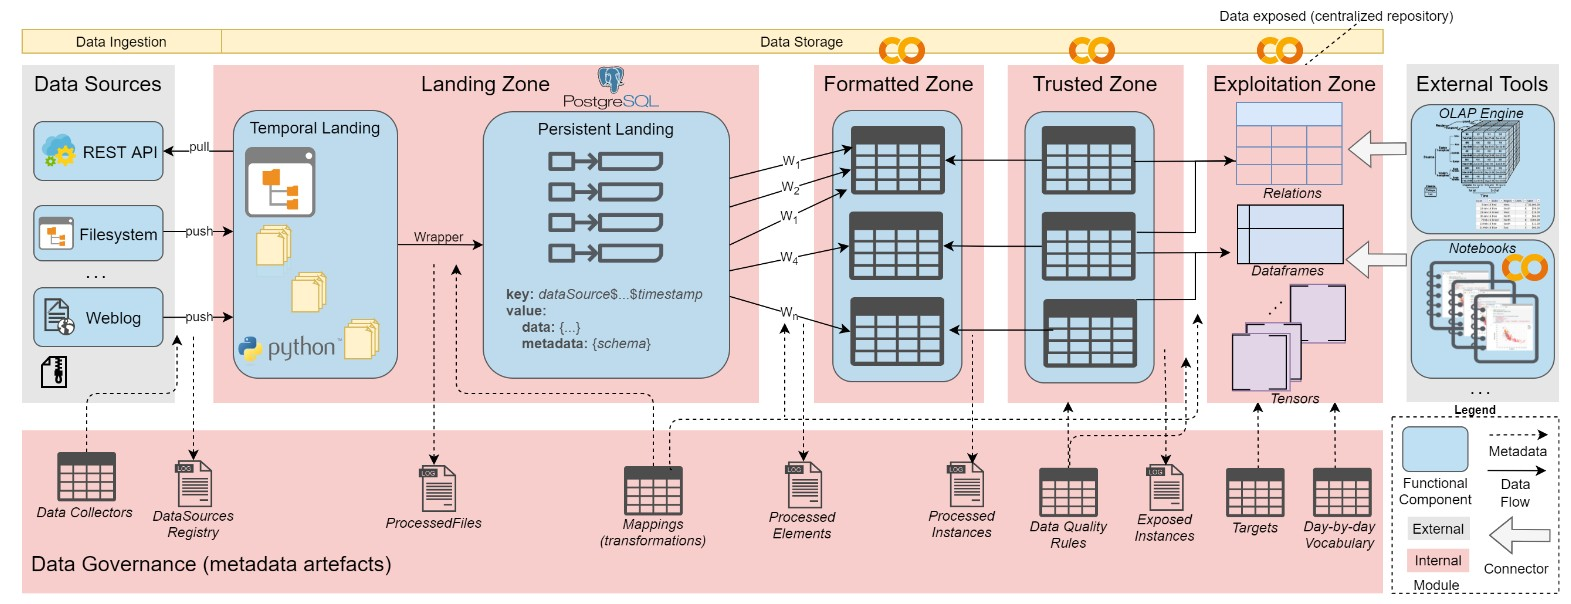
\includegraphics[width=\linewidth]{document/figures/data-management-backbone.jpg}
    \caption{data-management-backbone}
\end{figure}
\end{landscape}

The raw data is downloaded from the original sources through a script and stored in the temporal
landing zone. All our sources come in the form of zip files.

From there, using Python, we unzip the data and store the contents in the persistent landing zone.
For version managing, we add a checksum hash identifier alongside the timestamp from the ingestion in the folder name, following format: "<filename>-<sha256>-<ingestion\_timestamp>". This guarantees that there
are no collisions between different imports from the same source.

%\begin{minted}{javascript}
\begin{verbatim}
   {
     "contents": [
       "DEM_DATA_NATIONAL.csv",
       "DEM_LABEL.csv",
       "DEM_COUNTRY.csv",
       "DEM_README_RELEASE_2021_September.md"
     ],
     "dir": "./landing/persistent/extracted/DEM-070d666ac7d9d3c6c59b4905983e29768b02b9b9b684be97bc74afa1a41e42dd-1642969305.192381",
     "filename": "DEM.zip",
     "ingestion_time": "2022/01/23 21:21:45",
     "ingestion_timestamp": 1642969305.192381,
     "modification_time": "2022/01/22 17:26:34",
     "modification_timestamp": 1642868794.602461,
     "sha256": "070d666ac7d9d3c6c59b4905983e29768b02b9b9b684be97bc74afa1a41e42dd",
     "source": "../../../temporal/DEM.zip"
   }
\end{verbatim}

For each folder (which corresponds to an original data source file, we add a \texttt{metadata.json} file
which holds information on the data source from which the files in the folder were gathered.
This metadata files contain the filename, ingestion\_time, ingestion\_timestamp,
modification\_time, modification\_timestamp, sha256, source location and folder contents.

Additionally, we save join the metadata file from the result of each data ingestion on a global metadata file, gathering the info of all the files treated as well.

From there, we create the relational model and tables in a SQL schema and load all the CSV files into a Postgres database. The table names are versioned by the first four characters from the hash code identifier and timestamp. The table names follow the next format: "dataSource\_hashcode\_timestamp".
In order to import the data into the database, we hold information of how the sources correspond to the
databases. For this, we have one folder which contains the Schema of the databases to create in Postgres
and a file that tells for each source which of these schemas has to be applied.

For example, for table \texttt{CountryCodes} we have a file named \texttt{CountryCodes} in our
\texttt{sql\_spec} folder which contains the information on the columns:

\begin{verbatim}
"Country" integer PRIMARY KEY,
"Name" VARCHAR(50)
\end{verbatim}

And in \texttt{landing/spec\_tables.json} we have:
\begin{verbatim}
...
"country_codes": {
  "spec": "CountryCodes"
},
...
\end{verbatim}

This tells us that when ingesting files named \texttt{country\_codes}, the table should be processed
according to \texttt{CountryCodes}.

After this, in the trusted zone, we merge the different versions of the same source into a unified database per each source. As we have different timestamps for each source, we prioritize the data from the version that has been most recently uploaded. Additionally, in the trusted zone, a data quality analysis is performed. The script checks that the data is compliant with the rules standard rules defined for each column. Furthermore, we detect outliers and make profiling from each of the variables to assess their quality.